% !TeX root = ../main.tex
% Add the above to each chapter to make compiling the PDF easier in some editors.

\chapter{Approach}\label{chapter:approach}
One aim of this thesis is the prototypical implementation of heuristics to detect generated code which uses techniques of clone detection on the comments that are extracted from the source code. A list of patterns that detect generated code of several code generators is derived by means of the comments. Following a generator pattern repository has been created. The target of this repository is to provide a database of code generators and their respective characteristic generator pattern which identifies the source code containing it as generated.\\
We use a teamscale server to perform the basic analysis tasks on the specified projects.
\section{Use Teamscale as Lexer to extract Tokens}
The first step in the approach used in this paper is the lexical analysis of the source code included in the projects used as a benchmark. Teamscale comes with a multitude of lexers applicable for many different programming languages. The general workflow in this step is reading each source code file found in the project, perform the lexical analysis and tokenize the source code file into a sequence of logically coherent tokens representing the source code on a logical level. The tokens are saved server-side in the Teamscale instance.
% !TeX root = ../main.tex
% Add the above to each chapter to make compiling the PDF easier in some editors.

\begin{center}
	\begin{tikzpicture}[scale=2, node distance = 4cm, auto]
		\node [block] (init) {Source Code File};
		\node [block, right of=init] (lexer) {Lexical Analysis};
		\node [block, right of=lexer] (tokens) {Sequence of Tokens};
		% Draw edges
		\path [line] (init) -- (lexer);
		\path [line] (lexer) -- (tokens);
	\end{tikzpicture}
\end{center}

\section{Connect to the Teamscale server and retrieve comments}
\label{section:retrieveComments}
In the second step the tool written for this thesis connects to the Teamscale instance and retrieves the comments.\\
This has to be done in the following steps:
\begin{enumerate}
	\item Get the projects that are currently available in the Teamscale instance. 
	\item For each project retrieve the respective uniform paths to access the source code files on the server.
	\item For each uniform path retrieve the comments that are included in the respective source code file. In this step the server filters all tokens that are available for each file. The only important token class is the \textit{COMMENT} class, which itself contains the sub-classes shown in Table \ref{table:commentTypes}.
	\item The local file path of every source code file is retrieved from the server based on the uniform path. This will get important later in the evaluation.
	\item Each local file path gets associated to the respective list of comments.
\end{enumerate}

% !TeX root = ../main.tex
% Add the above to each chapter to make compiling the PDF easier in some editors.
\begin{center}
	\begin{tikzpicture}[scale=2, node distance = 3cm, auto]
		\node [block] (init) {Get Projects};
		\node [block, right of=init] (uniforms) {Retrieve Uniform Paths};
		\node [block, right of=uniforms] (filter) {Filter and Transfer Comments};
		\node [block, right of=filter] (local) {Get Local File Paths};
		\node [block, right of=local] (associate) {Associate Path to Comments};
		
		\path [line] (init) -- (uniforms);
		\path [line] (uniforms) -- (filter);
		\path [line] (filter) -- (local);
		\path [line] (local) -- (associate);
	\end{tikzpicture}
\end{center}
% !TeX root = ../main.tex
% Add the above to each chapter to make compiling the PDF easier in some editors.

\begin{table}[H]
	\caption{Comment types}
	\label{table:commentTypes}
	\begin{tabularx}{\textwidth}{l|L}
		\textbf{Token type} & \textbf{Example} \\
		\hline
		HASH\_COMMENT & \textit{\# Sample PHP script accessing HyperSQL through the ODBC extension module.}\\ 
		DOCUMENTATION\_COMMENT & \textit{/** Generated By:JJTree: Do not edit this line. */} \\ 
		SHEBANG\_LINE & \textit{\#!/usr/bin/env python } \\ 
		TRIPLE\_SLASH\_DIRECTIVE & \textit{/// <reference path="Parser.ts" />} \\ 
		TRADITIONAL\_COMMENT & \textit{/* Do not modify this code */} \\ 
		MULTILINE\_COMMENT & \textit{"""Testsuite for TokenRewriteStream class."""} \\ 
		END\_OF\_LINE\_COMMENT & \textit{// don't care about docstrings} \\ 
		SIX\_COLUMNS\_COMMENT & \textit{\dots} \\ 
	\end{tabularx} 
\end{table}

\section{Prepare comments for suffix tree clone detection}
Once the comments are received from the Teamscale server instance they have to get prepared to be usable in the suffix tree clone detection as introduced by Esko Ukkonen \cite{Ukkonen1995}\cite{Ukkonen1993}.\\
\subsection{Create thread for each source code file}
The step \ref{section:retrieveComments} produces a \textit{Map} in which every local path to a source code file is associated with its respective list of comments.
In the first part of the preparation one thread is generated for each source code file respective local file path. These threads will be responsible for the preparation of each single file and the results will be merged at the end.
\subsection{Remove unnecessary characters and whitespaces}
At first the comments are split at the linebreaks into single lines and leading and trailing whitespaces of each line are removed.\\
Susequent the comment enclosings are removed using a regular expression on every line to remove the language specific identifiers of comments. This regular expression is build from a list of regular expressions that represent the specific comment enclosings in the respective language.\\ 
These are concatenated with the \textit{OR}-operator to generate a generic regular expression for most programming language supported by Teamscale (\ref{section:teamscale}). Following this step the the leading and trailing whitespaces are removed again.\\
An overview of the regular expressions that are used in this step are shown in table \ref{table:commentEnclosings}.
% !TeX root = ../main.tex
% Add the above to each chapter to make compiling the PDF easier in some editors.

\begin{table}
	\caption[Comment enclosings]{Programming language specific regular expressions that represent comment identifiers (Escape characters are omitted).}
	\label{table:commentEnclosings}
	\begin{tabularx}{\textwidth}{l|L}
		\textbf{Programming language(s)} & Regular expression \\
		\hline
		C-like & ((\textasciicircum(/**|/*|*|//))|(*/)\$) \\
		Ada & (\textasciicircum(--)) \\
		Matlab & (\textasciicircum(\%)) \\
		Python & (\textasciicircum(\#)) \\
		XML & ((\textasciicircum(<!-{}-))|(-{}->)\$)
	\end{tabularx}
\end{table}

\subsection{Convert words into clone chunks}
The resulting lines of the previous step are again split into single words. Every word is at first checked if it holds valuable information for the approach. To check the value of each word it gets checked if it contains alphabetic letters \textit{(a-z, A-Z)} or digits. If a word only consists of nonalphabetic and no digits it gets sorted out \textit{(e.g. "-{}-{}-{}-{}-{}-{}-{}-")}.\\
The remaining words that bring a value to the approach are now converted into clone chunks. Therefore is added to every word the type of the comment, the offset and the linenumber of the comment and the local file path the comment originated from.\\
For an overview over these properties of a comment see \ref{section:token}.

\subsection{Add sentinels}
To prevent the suffix tree clone detection algorithm from intermixing the comments a sentinel gets added at the end of the list of clone chunks resulting from the previous steps. This is necessary due to the fact that the algorithm works an a single list of clone chunks that is build from merging all clone chunks from every comment.

\subsection{Merge thread results}
Once all threads are finished, resulting in all comments being converted into lists of clone chunks and sentinels being added to the end of each list, all lists get concatenated into one hugh list containing all words of the comments. On this list the suffix tree clone detection algorithm can now be applied.

\section{Build suffix tree}
Esko Ukkonen introduced an algorithm to construct suffix trees on strings in his paper for \textit{Algorithmica} in 1995 \cite{Ukkonen1995}. A suffix tree is a trie-like structure representing all suffixes of a string. To construct it a string gets processed symbol by symbol from the start to the end. The construction is based on the observation is that the suffixes of $T^i = t_1 \dots t_i$ can be obtained from expanding the suffixes of $T^{i-1} = t_1 \dots t_{i-1}$. \\
Figure \ref{fig:cacao} illustrates the algorithm an the word \textit{cacao}. For a deep insight on how the algorithm constructs the actual suffix tree see \cite{Ukkonen1995}.\\
For this thesis the algorithm has been expanded to work on any arbitrary datastructure. The simple observation behind this is that a string is just a list of characters. When building the suffix tree this list gets traversed from left to right and when adding a new character to the string suffix tree a simple equality check of the character and something {\Large expand here} is performed.\\
This property of the algorithm has been used to extend it to a generic version of it by allowing any list of data. The only mandatory property the data structure must provide is an equality function that can be evaluated in linear time to keep the linear time property of the algorithm. Therefore a function has been implemented that calculates the hash value of the data structure and performs a simple \textit{integer - integer} comparison that keeps the linear time property.
% !TeX root = ../main.tex
% Add the above to each chapter to make compiling the PDF easier in some editors.

\begin{center}
	\begin{figure}
		\centering
		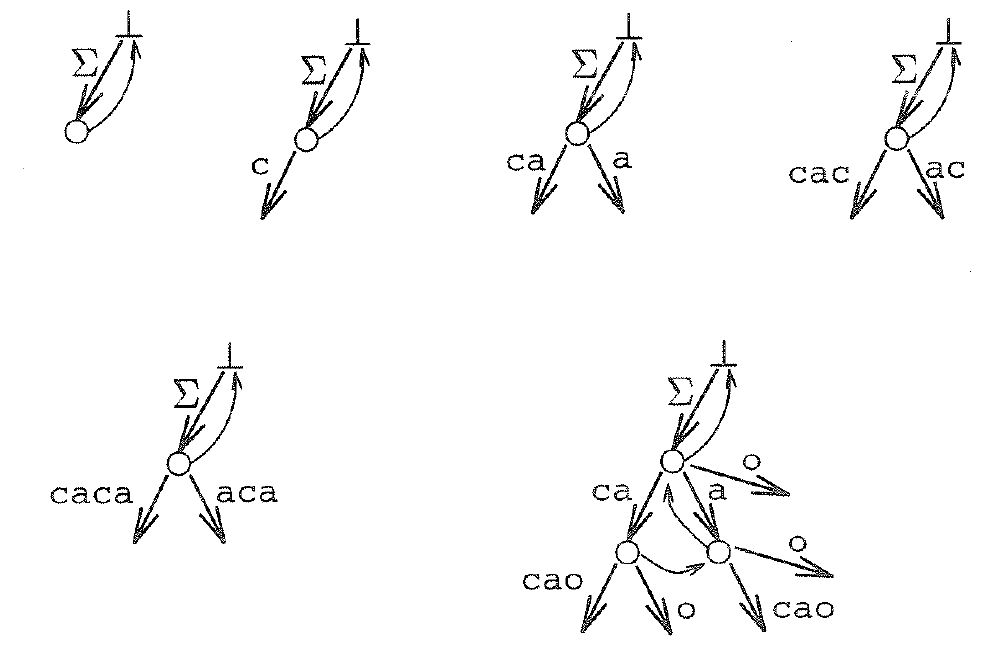
\includegraphics[width=0.9\linewidth]{figures/cacao}
		\caption[Suffix tree construction on the word \textit{cacao}]{Suffix tree construction on the word \textit{cacao}. \\
			\annotation{Maybe explain here. }}
		\label{fig:cacao}
	\end{figure}
\end{center}


\section{Find clones}
\section{Filter possibly generated clone results}
\section{Generate links to the files}
\section{Generation of a Generator-Pattern Repository}